% This is samplepaper.tex, a sample chapter demonstrating the
% LLNCS macro package for Springer Computer Science proceedings;
% Version 2.20 of 2017/10/04
%
\documentclass[runningheads]{llncs}
%
\usepackage{amsmath}
\usepackage{amssymb}
\usepackage{booktabs} % For pretty tables
\usepackage{caption} % For caption spacing
\usepackage{graphicx}
\usepackage{pgfplots}
\usepackage[all]{nowidow}
\usepackage[utf8]{inputenc}
\usepackage{tikz}
\usetikzlibrary{er,positioning,bayesnet}
\usepackage{multicol}
\usepackage{algpseudocode,algorithm,algorithmicx}
\usepackage{hyperref}
\usepackage[inline]{enumitem} % Horizontal lists
% Used for displaying a sample figure. If possible, figure files should
% be included in EPS format.
%
% If you use the hyperref package, please uncomment the following line
% to display URLs in blue roman font according to Springer's eBook style:
% \renewcommand\UrlFont{\color{blue}\rmfamily}
\graphicspath{{latex/}}
\newcommand{\card}[1]{\left\vert{#1}\right\vert}
\newcommand*\Let[2]{\State #1 $\gets$ #2}
\newcommand\qfrac[3][1pt]{\frac{%
		\ThisStyle{\addstackgap[#1]{\SavedStyle#2}}}{%
		\ThisStyle{\addstackgap[#1]{\SavedStyle#3}}%
}}


\newcommand{\F}{\ensuremath{\mathbb{F}}}
\newcommand{\B}{\ensuremath{\mathbb{B}}}
\newcommand{\LL}{\ensuremath{\mathbb{L}}}
\newcommand{\Me}{\ensuremath{\mathbb{M}_e^{\text{eff}}}}
\newcommand{\D}{\ensuremath{\text{D}}}
\renewcommand{\d}{\ensuremath{\text{d}}}
\pgfplotsset{compat=1.14}

\renewcommand{\topfraction}{0.85}
\renewcommand{\bottomfraction}{0.85}
\renewcommand{\textfraction}{0.15}
\renewcommand{\floatpagefraction}{0.8}
\renewcommand{\textfraction}{0.1}
\setlength{\floatsep}{3pt plus 1pt minus 1pt}
\setlength{\textfloatsep}{3pt plus 1pt minus 1pt}
\setlength{\intextsep}{3pt plus 1pt minus 1pt}
\setlength{\abovecaptionskip}{2pt plus 1pt minus 1pt}


\begin{document}
%
\title{A thermodynamically consistent multi-phase model of Extracellular Matrix}
%
\titlerunning{Mechanical Properties of ECM}
% If the paper title is too long for the running head, you can set
% an abbreviated paper title here
%
\author{Giulia Laura Celora}
%
%\authorrunning{F. Author et al.}
% First names are abbreviated in the running head.
% If there are more than two authors, 'et al.' is used.
%
\institute{Mathematical Institute University of Oxford}
%
\maketitle              % typeset the header of the contribution
%
\begin{abstract}

\end{abstract}
%
%
%
\section{Introduction}
There are now several studies supporting the central role of mechanical stimulus in tissue morphogenesis and homeostasis, alongside with biochemical signalling. \textit{In vitro} studies have shown that ECM rigidity and shear stresses can alone promote the transition to malignant phenotype of normal cells and consequently the growth of a tumour mass. Despite the well-known link between cell behaviour and mechanical stimuli, the lack of quantitative measurement has delayed our understanding of such phenomena. The development of new nanotechnology has now open to the possibility of measuring mechanical stresses by the use of external devices. Meanwhile, new techniques such as Atomic Force Microscopy (AFM) have been developed to measure the local mechanical properties of tissue, with atomic precision. Combining such information can boost our understanding and the development of a solid mathematical framework to describe tumour growth and exploit mechanics to improve and revolutionise current therapy against cancer. 

The aim of coupling micro-environment and cell behaviours requires a clear understanding of both and the investigation of phenomena occurring at different time and spacial scales. In this work we focus on the Extracellular Matrix (ECM), the external network of polymers supporting cells in tissues. Its mechanical properties, in particular its stiffness, contribute to determine the response of tissues to external mechanical stimuli. By controlling the composition of the matrix, its properties can be tuned to meet the function of a specific tissues. 

Experiments have shown that tumour development is associated to a stiffening of the tissue compared to the surrounding healthy one, despite the fact that tumour cells themselves are usually softer than normal ones. Such contradiction is just apparent, as ECM can account for such resistance to mechanical stimuli. As a result, cells are exposed to higher compressive stresses which can select for more aggressive and invasive phenotype of cancer cells, as well as favour the collapse of blood vessels and impede the diffusion of substances in the extra-cellular environment ultimately decreasing the efficacy of numerous therapies.

Usually approach to the modelling of solid tumour is the use of multi-phase theory, according to which tumour are equivalent to material consisting of a solid matrix of cells and ECM, and an interstitial fluid phase. Besides involving the use of fundamental laws such as conservation of mass and momentum, the formulation of the model requires the use of several constitutive equation for each of the phase considered. These dictate the macroscopic behaviour of the system and thus heavily affect the prediction of the model, and are usually based on experimental result and have thus a limited range of applicability. Having a more fundamental description of the system requires instead deriving such properties based on the microscopic behaviour of the system.   As mentioned before, there is little understanding on the properties of the fundamental components of the ECM.

\section{Non Equilibrium Thermodynamics.}
\label{secNET}
While equilibrium thermodynamics successfully apply to the description of ideal process, real processes are irreversible. In this cases, the change in entropy $\d S$ can result from the reversible exchange of energy and matter with the external environment, $\d_eS$ or the internal dissipation od energy during the process, $\d_iS$ \cite{NET}:
\begin{equation}
\d S = \d_eS + \d_iS, \hspace{5mm} \d_eS= \frac{\d Q}{T},
\end{equation}
where $Q$ is the amount of energy added to the environment and $T$ is the temperature. 
According to the second law of thermodynamics, which applies universally to any system or subsystem, $\d S_i\ge 0$.

For the purpose of this study, we will focus on isothermal process, i.e. $T=const$. Under this assumption, as derived by Gurtin in \cite{GURTIN}, the second law of thermodynamics is equivalent to the following \textit{energy imbalance inequality}:
\begin{equation}
\frac{\d}{\d t} \left\{\int_R \psi \right\}\leq W(R) + M(R) \label{energyin}
\end{equation}
where $R$ is a arbitrary control volume of the system, $\psi$ is the Helmholtz free energy, $W(R)$ is the rate at which the environment does work on $R$ and $M(R)$ is the inflow of mass due to transport. It is important to note that the energy inequality~(\ref{energyin}) holds for any isothermal process, independently of the specific physical system involved. Consequently, there is a constraint on the form the function $\psi$ can assume and how this can depend on the thermodynamic variables describing the system. 

The major focus of non-equilibrium thermodynamics is in defining the precise form of $\d_i S$, which, unlike $\d_e S$ is not a state function, but depends on the specific transformation applied to the system. This is introduced in the theory with the concepts of \textit{thermodynamic forces} $F_m$ (cause) and \textit{thermodynamic fluxes} $J_m$ (effect) has been introduced, so that $\d_iS$ has the form:

\begin{equation}
\d_iS = \sum_m F_m J_m.
\label{2law}
\end{equation}

Different relation between forces and fluxes have been proposed in the literature giving rise to a variety of theory, each with its specific domain of applicability \cite{NET}. In our study we will focus on \textquotedblleft Classical Irreversible Thermodynamics'' (CIT) which was pioneered by Onsager \cite{onsager} and Prigogine \cite{prigogine} in the first half of the 20th century. This is built on three major assumptions:
\begin{itemize}
	\item[1.] \textit{Local Equilibrium Hypothesis}: thermodynamic variables are locally well-defined;
	\item[2.] \textit{Linear Relation between forces $F$ and fluxes $J$}:
	\begin{equation}
	J_m = \sum_k L_{mk} F_k,\label{lin}
	\end{equation}
	where the constant $L_{mk}$ are referred to as \textbf{phenomenological coefficients};
	\item[3.] \textit{Microscopic Reversibility}: time reversibility of processes at the micro-scale. 
\end{itemize}

Despite the wide range of applicability of such theory, this does not apply to the domain of far-from equilibrium thermodynamics, for the linear approximation breaks down. It is still under debate which range of physical phenomena lie in the domain of applicability of CIT, particularly in the novel realm of active matter, where experimental validation of theories still lacks.

\section{Extracellular Matrix.}
Despite the tissue-specific nature of Extracellular Matrix (ECM), this is mainly composed of a network of collagen fibrils entangled with charged chains of glycosaminoglycans (GAGs). While collagen is mainly responsible for the mechanical behaviour of the tissue, GAGs can imbibe water, giving ECM the ability to swell while maintaining its structural integrity. As a result, the ECM behave as a polyelectrolyte gel \cite{ecm,ecm2}. Besides being largely present in the natural world, synthetic polyelectrolytes are currently employed for a wide range of applications, such as drug delivery, biomedical devices, scaffolds for tissue engineering and soft robotics [ADD CITATIONS]. The increasing popularity of such material has boost the development of mathematical model of such systems, in particular focusing particularly on the their swelling and plastic behaviours [ADD CITATIONS].

There is now compelling evidence that the relaxation of stress in polymer gels, and thus in ECM is governed by the interplay of the poroelastic and viscoelastic nature of the gel. While the first determines the long range motion of solvents, visco-elastic dominates the stress relaxation dynamics at the microscopic level. Being the same level at which cells probe their environment, this suggests that the visco-elastic properties of the ECM might play a role in determining cell response [ADD ARTICLE IN NOTE AS CITATION].


\section{Model Development}
\subsection{Conservation Law.}

The ECM is here considered as a three-phase medium composed of a solid polymer network with fixed charges, a solvent (i.e. water molecules) and solutes (freely moving charges).

We here assume that the deformation of the ECM corresponds to the one of the solid network. As the tissue deform, the material element originally located at $\mathbf{X}$ in the initial configuration $\mathcal{B}_0$ is displaced to the point $\mathbf{x}$ in the current configuration $\mathcal{B}$. Such transformation is described by the deformation gradient $\F= \partial \mathbf{x}/\partial \mathbf{X}$, while the information about its change in the ECM volume due to swelling is encoded in $J= \det \F$. Since we assume the solid phase to be incompressible, any change in the volume can only be related to the migration of solvent and solutes molecules, whose nominal concentrations will be denoted by $C_s$ and $C_i$ respectively, $i=1,\ldots,N$ with $N$ number of free ion species. This lead to the molecular incompressibility condition:

\begin{equation}
 J= 1 + v_s C_s +\sum\limits_{i=1}^{N} v_i C_i
 \label{comp}
\end{equation}
where $v_m$ are the characteristic molecular volume of each species. As common in tissue modelling, we will here assume that the contribution of ions to the volume is negligible so that Equation~(\ref{comp}) reduces to:
\begin{equation}
J=1+v_s C_s.
\end{equation} 

The volume fractions of fluid $\phi_f$ and solid $\phi_n$ phases in the gel are thus be defined as:
\begin{equation}
\phi_f -= \frac{v_sC_s}{1+v_sC_s}, \qquad \phi_n = \frac{1}{1+v_sC_s}.
\end{equation}
While $C_m$ denote the number of each phase molecule per unit volume in the initial configuration, the actual concentration in the current state is denoted by $c_m=C_m/J$. Note that throughout this work we will be using $i=1,\ldots,N$ for denote only the concentration of ionic species, while $m\in\left\{s,1,\ldots,N\right\}$ to refer to both the solvent and solutes.

Mass conservation must apply to all mobile species and in the initial configuration these read:
\begin{equation}
\dot{C}_m + \nabla_0 \cdot \mathbf{J}_m = 0, 
\end{equation}
where $\mathbf{J}_m$ is the nominal flux per unit area in the dry state and $\nabla_0$ denote the gradient in the Lagrangian coordinate $\mathbf{X}$. Their counterparts in the actual configuration are denoted by $\mathbf{j}_m$ and $\nabla$ and are defined by the flow rule:
\begin{equation}
\mathbf{J}_m = J \F^{-1} \mathbf{j}_m, \qquad \nabla_0 (\cdot) = \F^{T} \nabla(\cdot).
\end{equation}

We also neglect any effect due to inertia, or any internal volume force so that the conservation of momentum for the gel reads:
\begin{gather}
\nabla_0 \cdot \mathbb{S}=0\\
\end{gather}
where $\mathbb{S}$ is the first Piola-Kirchoff tensor, which is related to the Cauchy stress tensor $\mathbb{T}$, as:
\begin{equation}
\mathbb{T} = J^{-1}\mathbb{S}\F^T.
\end{equation}

The presence of free moving ions generates and electric field which is denoted by $\mathbf{E}$ and $\mathbf{e}$ in the initial and current configuration respectively. Introducing the electrostatic potential $\Phi$, we have that:
\begin{equation}
\mathbf{E}= -\nabla_0 \, \Phi, \hspace{8mm} \mathbf{e}= - \nabla \, \Phi.
\end{equation}
As the gel is here considered to be a dielectric material, the presence of the field induces an electric displacement, which must satisfy Gauss law of electrostatics:
\begin{equation}
\nabla_0 \cdot \mathbf{H}= Q,
\label{gauss}
\end{equation}
where $\mathbf{H}$ is the nominal electric displacement and $Q$ is the local total charge, which accounts for both fixed and moving charges:
\begin{equation}
Q = e\left(\sum\limits_{i} z_i C_i+z_f C_{f}\right)\, , 
\end{equation}
where $e$ is the elementary charge, $C_f$ is the concentration of fix charges and $z_m$ is the valence of the corresponding charged species. Note that $C_f$ here corresponds to the concentration of GAGs, which is only a fraction of $C_s$. As for above, we can move from nominal quantities to the corresponding value in the current configuration by applying the following rules:

\begin{eqnarray}
\mathbf{H} = J \mathbf{h}\F^{-T},\\
\mathbf{E} = \F^T \mathbf{e},
\end{eqnarray}
where $\mathbf{h}$ is the electric displacement in the current configuration.
\subsection{Kinematics.}
As in [SARAH PAPER], we here consider that the initial state of the system $\mathcal{B}_0$ corresponds to the dry state of the gel. At any time $t$, the actual configuration of the body is $\mathcal{B}_t$. In this section, we want to focus on the rule according to which the body deforms from $\mathcal{B}_0$ to $\mathcal{B}_t$, which depends on the properties of the system studied. In our case, we consider a poro-visco-elastic material. As shown in Figure \ref{deformation}, there are two mechanisms that can contribute to the change in the body conformation: a volume preserving viscous deformation and long range transport of fluid that leads to swelling. 

\begin{figure}
	\centering
	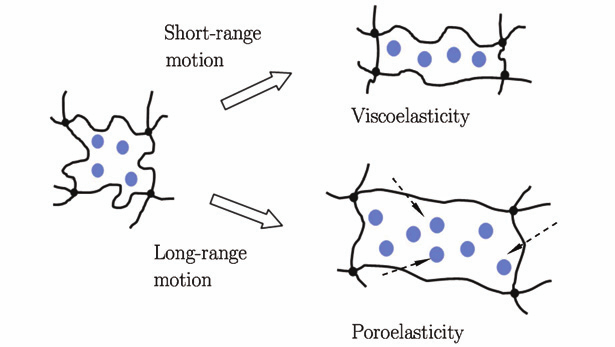
\includegraphics[scale=0.325]{images/visco_poro}
	\caption{Illustration of the molecular processes which account for a gel deformation: viscosity is related to change in the conformation of the network which results in short-range movement of fluid relative to the polymers; poro-elasticity is instead responsible for the long-range diffusion of solvent molecules in the gel/tissue. Reproduced from \cite{viscoporo}.}
	\label{deformation}
\end{figure}
 
We are here interested in the coupling of this two phenomena and how information from experiment at different spatial and temporal scale can be coupled. To do so, we will here present two different approaches that have been proposed in the literature to describe the complex mechanics of hydrogels. In particular, nanoscale rheological testing with AFM usually rely on a 1D \textit{Standard Linear Solid} model, as the one shown in Figure \ref{fig1}, to fit the experimental data \cite{Article1,viscoporo}.  

\begin{figure}[h!]
	\hspace{10mm}
	\def\svgwidth{0.95\linewidth}
	\input{latex/images/model1.pdf_tex}
	\caption{Rheological model 1 and corresponding deformation decomposition.}
	\label{fig1}
\end{figure}

As pointed out by Hu et~al. \cite{viscoporo}, AFM measurements with nano-scale beads allow to capture the viscoelastic relaxation dynamics. But given the short length scale considered in the experiment, poroelastic relaxation is too fast to be captured. On the other hand, when considering larger time and spatial scale, such in standard compression test, the situation is reversed and what can be measure is the poroelastic dynamics. In this regime, the system can be well approximated by a poro-hyperelastic model.
\subsection{Energy Balance Inequality.}
As mentioned in Section \ref{secNET}, the energy imbalance inequality impose restriction on the nature of the free energy $\psi$ of the system depending on how this exchanges energy and mass with the environment. Considering a control volume $R$ in the reference configuration, the system exchanges mass due to diffusion of each mobile species, so that $M(R)$ is given by:
\begin{equation}
M(R)= \sum\limits_{m=s,1,\ldots,N} - \int_{\partial R} \mu_m \,\mathbf{J}_m \cdot \mathbf{n} 
\end{equation}
where $\mathbf{n}$ is the unit normal vector to the surface $\partial R$ and $\mu_m$ is the chemical potential associated with each species. Widely used in the thermodynamics of mixture, the chemical potential is a measure of the rate of change in free energy associated with adding to a unit volume one more molecule. The work done on $R$ in the original configuration per unit time $W(R)$ is instead made up of two contributions, the electrical $W_{el}(R)$ and mechanical work $W_{mec}(R)$. Following [ADD CITATION DROZDOV,inhomogeneous swelling ph-responsive gel], $W_{el}(R)$ is defined as:
\begin{equation}
W_{el}(R) = -\int_{\partial R} \Phi\, \dot{\mathbf{H}}\cdot \mathbf{n}
\end{equation}
As suggested by Gurtin \cite{GURTIN}, when accounting for the mechanical work, we consider also the effect of micro-stresses $\boldsymbol{\epsilon}$, which arise due to the system heterogeneity [ADD CITATION, The Interactions of Composition and Stress 
in Crystalline Solids]. As before we consider that the dominant contribution is related to the solvent, so that:
\begin{equation}
W_{mec}(R) = \int_{\partial R} \left(\boldsymbol{\xi}\cdot \mathbf{n}\right)\dot{C}_s + \int_{\partial R} \mathbb{S}\mathbf{n} \cdot \dot{\mathbf{u}}
\end{equation}
where $\mathbf{u}= \mathbf{x}-\mathbf{X}$ is the displacement vector, which is related to the deformation tensor, $\F=\mathbb{I}-\nabla_0 \mathbf{u}$. Substituting this result back into the energy imbalance, see Equation~(\ref{energyin}) and using the divergence theorem we obtain the following integral inequality:
\begin{equation}
\int_R \dot{\psi} - \mathbf{E}\cdot \dot{\mathbf{H}} \, + \, \sum\limits_{i=1}^{N} \left[e \Phi  z_i \dot{C}_i+ \nabla_0 \left(\mu_i \mathbf{J}_i \right)\right] + \nabla_0 (\mu_s \mathbf{J}_s- \boldsymbol{\xi}\dot{C}_s -\mathbb{S}^T\mathbf{\dot{u}}) \leq 0 
\end{equation}
Since the above inequality must hold for any choice of the volume $R$, the constraint must hold locally. So that:
\begin{equation}
\dot{\psi} - \mathbf{E}\cdot \dot{\mathbf{H}} \, + \, \sum\limits_{i=1}^{N} \left[e \Phi  z_i \dot{C}_i+ \nabla_0 \left(\mu_i \mathbf{J}_i \right)\right] + \nabla_0 (\mu_s \mathbf{J}_s- \boldsymbol{\xi}\dot{C}_s -\mathbb{S}^T\mathbf{\dot{u}}) \leq 0. 
\end{equation}
Further accounting for the balance laws presented in the previous section, we obtain that:
\begin{equation}
\begin{aligned}
\dot{\psi} - \mathbf{E}\cdot \dot{\mathbf{H}} \, + \, \sum\limits_{i=1}^{N} \left[e \Phi  z_i - \mu_i\right] \dot{C}_i - (\mu_s + \nabla_0 \cdot \boldsymbol{\xi})\,\dot{C}_s -\mathbb{S}:\dot{\F}\\
-\boldsymbol{\xi} \cdot \nabla_0 \, \dot{C}_s + \sum\limits_{m} \nabla_0 \, \mu_m \cdot \mathbf{J}_m \leq 0.
\end{aligned} 
\end{equation}

\bibliographystyle{splncs04}
\bibliography{latex/ref}
%
\end{document}
